%%%%%%%%% Notes %%%%%%%%%

%%%%%%%%% Packages %%%%%%%%%
\documentclass[aspectratio=43]{beamer}
\usepackage[T1]{fontenc}
\usepackage{derivative}
\usepackage{pgfpages}

%%%%%%%%% Packages setup %%%%%%%%%
\setbeameroption{show notes on second screen}
%\setbeameroption{show only notes}
%\setbeamerfont{note page}{size=\tiny}
\setbeamercolor{note page}{bg=white, fg=black}
\setbeamercolor{note title}{bg=white!99!black, fg=black}
\usetheme{Hannover}
\usecolortheme{spruce}
\graphicspath{{./figures/}{../report/figures/}}

\newcommand{\zTOA}{z_\text{TOA}}
\newcommand{\PTOA}{P_\text{TOA}}
\newcommand{\deltaTOA}{\delta_\text{TOA}}

%%%%%%%%% Document informations %%%%%%%%%
\title{Radiative-convective equilibrium in a grey atmosphere}
\author{Marco Casari}
\date[03/10/2023]{Complex systems in climate physics, 3 October 2023}
\institute[UniTo]{University of Turin}

%%%%%%%%% Document %%%%%%%%%
\begin{document}
\begin{frame}
  \titlepage
  \note{
    \begin{itemize}
      \item A radiative-convective model is used to study a grey atmosphere.
      \item Comparison between numerical and analytical solutions is possible in radiative equilibrium.
    \end{itemize}
  }
\end{frame}

\section{Introduction}
\begin{frame}{Introduction}
  \begin{itemize}
    \item<1-> Average vertical temperature profile $T(t, z)$ of atmosphere.
    \note[item]<1->{The analysed quantity is the atmospheric temperature profile averaged over all latitudes and longitudes.}
    \item<2-> Radiative Transfer Equation (RTE).
    \note[item]<2->{RTE describes radiative processes.}
    \item<3-> Fluid dynamics equations.
    \note[item]<3->{Fluid dynamics equations describe convective processes.}
  \end{itemize}
\end{frame}

\begin{frame}{Hypotheses}
  \begin{itemize}
    \item<1-> Thermodynamic energy equation in Local Thermodynamic Equilibrium (LTE):
      \begin{equation}
        \label{eq:temperature_derivation}
        \pdv{T}{t} = -\frac{1}{\varrho c_P} \pdv{q}{z}
        \quad .
      \end{equation}
    \note[item]<1->{Thermodynamic energy equation describes average vertical temperature profile.}
    \item<2-> Radiative-convective equilibrium.
    \note[item]<2->{The study is conducted on an atmosphere in radiative-convective equilibrium.}
    \item<3-> Grey atmosphere.
    \note[item]<3->{Quantities do not depend on the frequency of electromagnetic radiation.}
  \end{itemize}
\end{frame}

\begin{frame}{Additional hypotheses}
  \begin{itemize}
    \item<1-> Hypotheses on the planet.
    \note[item]<1->{Diurnal cycle, constant irradiance, constant Bond albedo, surface emits blackbody radiation, constant gravitational acceleration.}
    \item<2-> Hypotheses on the composition of atmosphere.
    \note[item]<2->{Hydrostatic equilibrium, constant specific heat at constant pressure, scattering is neglected, absorption coefficient depends only on altitude, constant mass attenutation coefficient, ideal gas.}
    \item<3-> Hypotheses on total heat flux.
    \note[item]<3->{Heat flux determined only by radiative and convective processes, two-stream approximation, numerical correction for convection.}
    \item<3-> Resulting thermodynamic energy equation:
      \begin{equation}
        \label{eq:temperature}
        \pdv{T}{t} = -\frac{1}{\varrho c_P} \pdv*{\big( E_\text{U} - E_\text{D} \big)}{z}
        \quad .
      \end{equation}
  \end{itemize}
\end{frame}

\begin{frame}{Vertical coordinates}
  \begin{itemize}
    \item Relation between pressure and altitude:
      \begin{equation}
        \label{eq:pressure_altitude}
        P(z) = P_\text{g} \exp{\bigg( - \frac{z - z_\text{g}}{z_0} \bigg)}
        \quad .
      \end{equation}
    \note[item]{Obtained from hydrostatic equilibrium and ideal gas law.}
    \item Relation between optical depth and pressure:
      \begin{equation}
        \label{eq:optical_depth_pressure}
        \delta(P) = \frac{\mu_\text{m}}{g} (P - \PTOA)
        \quad .
      \end{equation}
    \note[item]{Obtained from definition of optical depth, hydrostatic equilibrium and hypotheses on attenutation coefficient.}
    \item Relation between optical depth and altitude:
      \begin{equation}
        \label{eq:optical_depth_altitude_2}
        \delta(z) = \frac{\mu_\text{m}}{g} \bigg( P_\text{g} \exp{\bigg( - \frac{z - z_\text{g}}{z_0} \bigg)} - \PTOA \bigg)
        \quad .
      \end{equation}
    \note[item]{Obtained by combining relations~\eqref{eq:pressure_altitude} and~\eqref{eq:optical_depth_pressure}.}
  \end{itemize}
\end{frame}



\section{Radiative equilibrium}
\begin{frame}{Equations in radiative equilibrium}
  \begin{itemize}
    \item<1-> RTE for non-scattering medium in LTE:
      \begin{equation}
        \label{eq:RTE_analytical}
        \frac{1}{\mu} \pdv{L}{z} = B_\nu - L
        \quad .
      \end{equation}
    \note[item]<1->{RTE describes radiance in a medium.}
    \item<2-> Integration over frequency and solid angle.
    \item<2-> Diffusion approximation: $\delta' = D \delta$.
    \note[item]<2->{To describe irradiances, RTE is integrated over the whole spectrum of radiation and over the solid angle of a hemisphere.}
    \item<3-> Equations for irradiances:
      \begin{align}
        \label{eq:irradiance_upward}
        - \pdv*{E_\text{U}(t, \delta')}{\delta'} & = \sigma T(t, \delta')^4 - E_\text{U}(t, \delta') \quad , \\
        \label{eq:irradiance_downward}
        \pdv*{E_\text{D}(t, \delta')}{\delta'} & = \sigma T(t, \delta')^4 - E_\text{D}(t, \delta')
        \quad .
      \end{align}
    \note[item]<3->{Equations for irradiances and temperature are written in terms of $\delta'$.}
  \end{itemize}
\end{frame}

\begin{frame}{Initial Value Problem}
  \begin{itemize}
    \item<1-> Steady state.
    \note[item]<1->{Analytical solutions are found for temperature at the steady state.}
    \item<2-> Initial conditions on irradiances:
      \begin{align}
        \label{eq:initial_downward}
        E_\text{D}(0) = 0 \quad , \\
        \label{eq:initial_upward}
        E_\text{U}(0) = S_\text{t}
        \quad .
      \end{align}
    \note[item]<2->{At TOA downward irradiance does not deposit energy and radiative equilibrium fixes upward irradiance, i.e. outgoing longwave radiation.}
    \item<3-> Additional relations:
      \begin{align}
        \label{eq:irradiance_steady_state}
        \odv*{\big( E_\text{U}(\delta') - E_\text{D}(\delta') \big)}{\delta'} = 0
        \quad , \\
        \label{eq:irradiance_steady_state_solution}
        E_\text{U}(\delta') - E_\text{D}(\delta') = S_\text{t}
        \quad .
      \end{align}
    \note[item]<3->{Hypotheses of atmosphere in radiative equilibrium at all altitudes and atmopshere transparent to radiation coming from outside the planet are equivalent to hypotheses of atmopshere in radiative equilibrium at TOA and steady state.}
    \item<4-> Initial condition on temperature:
      \begin{equation}
        \label{eq:initial_temperature}
        T(0) = \bigg( \frac{S_\text{t}}{2 \sigma} \bigg)^\frac{1}{4}
        \quad .
      \end{equation}
    \note[item]<4->{Initial condition on temperature is obtained by combining all conditions on irradiances.}
  \end{itemize}
\end{frame}

\begin{frame}{Analytical solution}
  \begin{itemize}
    \item Temperature:
      \begin{equation}
        \label{eq:temperature_analytical_solution}
        T(\delta) = \bigg( \frac{S_\text{t}}{2 \sigma} (1 + D \delta) \bigg)^\frac{1}{4}
        \quad .
      \end{equation}
    \item Irradiances:
      \begin{align}
        \label{eq:irradiance_upward_solution}
        E_\text{U}(\delta) & = \frac{S_\text{t}}{2} (2 + D \delta) \quad , \\
        \label{eq:irradiance_downward_solution}
        E_\text{D}(\delta) & = \frac{S_\text{t}}{2} D \delta
        \quad .
      \end{align}
  \end{itemize}
\end{frame}

\begin{frame}{Numerical solution}
  \begin{itemize}
    \item Normalisation:
      \begin{equation}
        \label{eq:normalisation}
        Y_0 = \frac{T^4}{T_0^4}
        \quad , \quad
        Y_1 = \frac{E_\text{U}}{S_\text{t}}
        \quad , \quad
        Y_2 = \frac{E_\text{U}}{S_\text{t}}
      \end{equation}
    \item Resulting system of ODEs:
      \begin{equation}
        \label{eq:numerical_steady_state}
        \left\{
        \begin{array}{@{}l@{}}
          \odv{Y_0}{\delta} = \frac{D}{2} \\[0.5em]
          \odv{Y_1}{\delta} = D (Y_1 - Y_0) \\[0.5em]
          \odv{Y_2}{\delta} = D (Y_0 - Y_2)
        \end{array}
        \right.
        \quad .
      \end{equation}
    \item Runge-Kutta method of order 4.
    \item Non-uniform step size.
  \end{itemize}
\end{frame}

\begin{frame}{Errors of numerical solutions}
  \begin{center}
    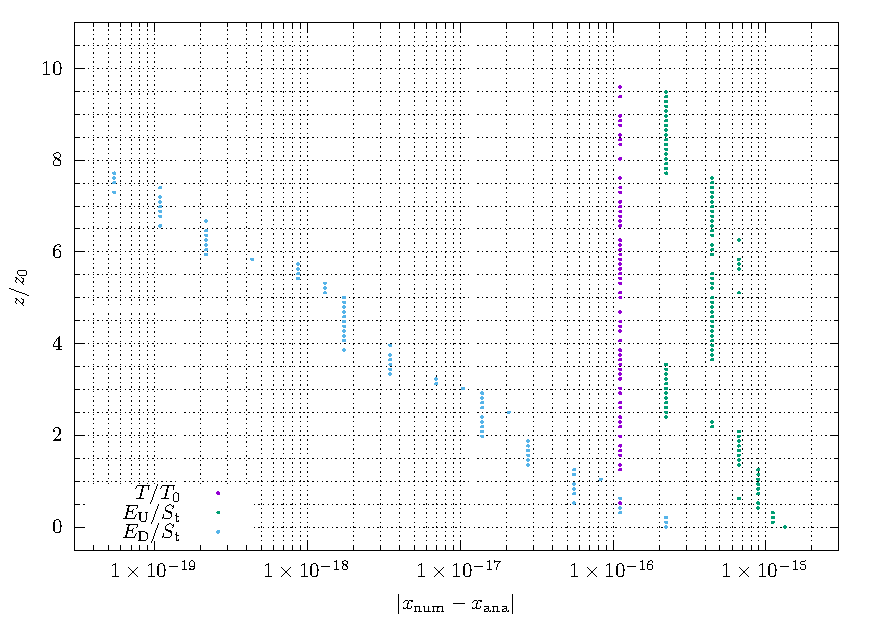
\includegraphics[keepaspectratio=true,width=0.9\textwidth]{errors}
  \end{center}
  \note{
    \begin{itemize}
      \item Errors between numerical and analytical solutions of a grey atmosphere in radiative equilibrium, assuming steady state. Points at some altitudes are not shown because their value is exactly 0.
      \item Errors are compatible with 0 based on precision of double-precision floating-point numbers.
    \end{itemize}
  }
\end{frame}

\begin{frame}{Stability analysis}
  \begin{center}
    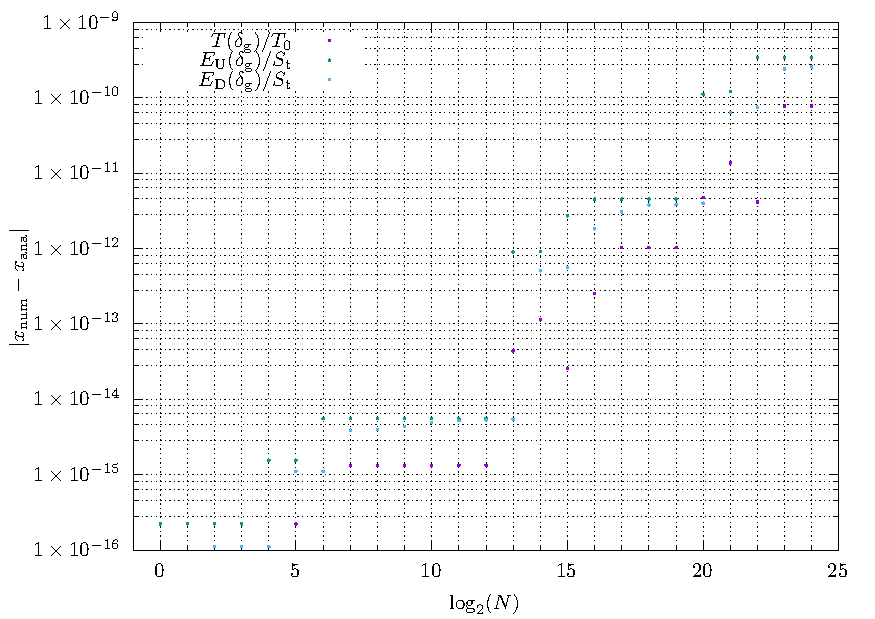
\includegraphics[keepaspectratio=true,width=0.9\textwidth]{stability}
  \end{center}
  \note{
    \begin{itemize}
      \item Stability of numerical solution for ODEs system in radiative equilibrium with respect to spatial grid size. Errors are negligible up to 4096 layers, then error propagation dominates reducing the precision of the method. Missing points have value 0.
      \item Errors are evaluated as absolute differences between numerical and analytical values at ground level of each normalised function.
    \end{itemize}
  }
\end{frame}

\begin{frame}{Time integration}
  \begin{itemize}
    \item<1-> Iterative procedure.
    \item<2-> Additional normalisation:
      \begin{equation}
        \label{eq:temperature_normalisation}
        Y_3 = \frac{T}{T_0}
        \quad .
      \end{equation}
    \item<3-> Resulting system of PDEs:
      \begin{equation}
        \label{eq:numerical_radiative_equilibrium}
        \left\{
        \begin{array}{@{}l@{}}
          \pdv*{Y_3(t, \delta)}{t} = \frac{\mu_\text{m} S_\text{t}}{c_P T_0} \pdv*{(Y_1(t, \delta) - Y_2(t, \delta))}{\delta} \\[0.5em]
          \pdv*{Y_1(t, \delta)}{\delta} = D (Y_1(t, \delta) - Y_3(t, \delta)^4) \\[0.5em]
          \pdv*{Y_2(t, \delta)}{\delta} = D (Y_3(t, \delta)^4 - Y_2(t, \delta))
        \end{array}
        \right.
        \quad .
      \end{equation}
    \item<3-> Euler method for temporal integration.
    \item<3-> Constant time step.
  \end{itemize}
\end{frame}

\begin{frame}{Errors of time integration at steady state}
  \begin{center}
    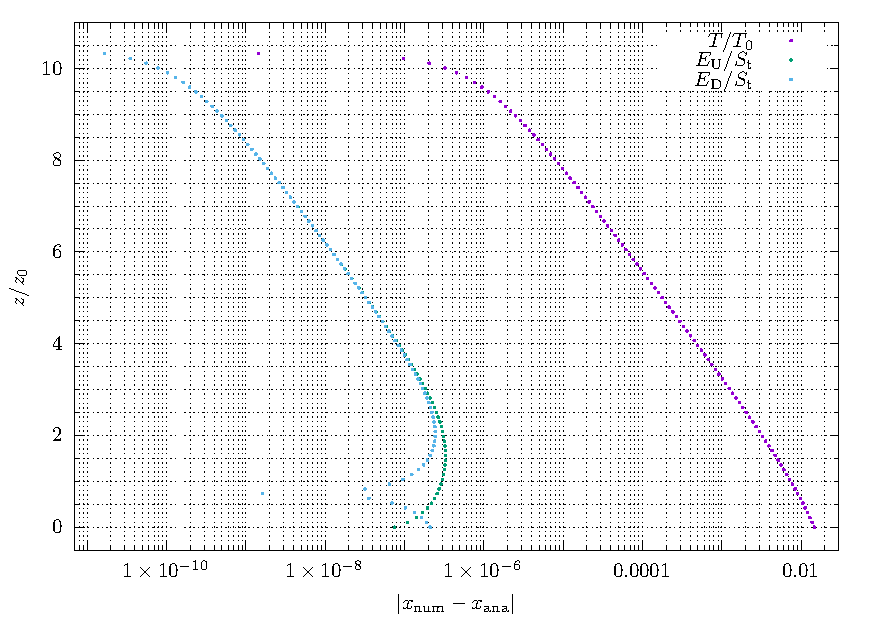
\includegraphics[keepaspectratio=true,width=0.9\textwidth]{errors_PDE}
  \end{center}
  \note{
    \begin{itemize}
      \item Errors between numerical and analytical solutions of a grey atmosphere in radiative equilibrium. Steady state is reached throught iterative temporal and spatial integrations. Precision is reduced by propagation of errors during successive iterations. Points at TOA are omitted being compatible with 0 within precision of double-precision floating-point numbers.
      \item Time step is chosen arbitrarily to reduce the errors of irradiances below the precision of numeric values outputs.
    \end{itemize}
  }
\end{frame}



\section{Radiative-convective equilibrium}
\begin{frame}{Radiative-convective equilibrium}
\end{frame}



\section{Conclusion}
\begin{frame}{Conclusion}
  % MC put conclusive summary with items.
%  \vfill
%  \onslide<2->{
%    \centering
%    \huge
%    Thank you
%  }
\end{frame}
\end{document}
